\documentclass{article}
\usepackage{graphicx}
\graphicspath{{./figure/}}  % папки с картинками

\begin{document}

\begin{titlepage}
	
	\begin{center}
		
		\vspace{1cm}

		{\Huge \textsc{U s e r' s \, \, G u i d e}}
		
		
		\vspace{1cm}
		\hrulefill
		\vspace{1cm}
		
		{\Huge \textbf{GUI4DFT \, \, 1.0}}
		
		\vspace{1cm}
		\hrulefill
		\vspace{0.5cm}
		
		%{\Large \printdate}
		
		\vspace{1.5cm}
		{\Large https://github.com/sozykinsa/GUI4dft}
		
		\vspace{2.5cm}
		%Steering Committee:
		\vspace{1.0cm}
		
		\begin{tabular}{ll}
			
			Sergey Sozykin  \\  %&
			\textit{South Ural State University, Chelabinsk, Russia} \\
			
			% ...
						
		\end{tabular}
		
	\end{center}
	
\end{titlepage}

	
	
\section{About GUI4DFT program}

GUI4DFT (Graphical User Interface for support of Density Functional Theory calculations) -- the SIESTA oriented GUI (see Fig.\ref{fig:mainwindow}). It is a cross-platform program. The program was tested in Windows, Mac OS and Ubuntu operating systems.

\begin{figure}[h!]
	\centering
	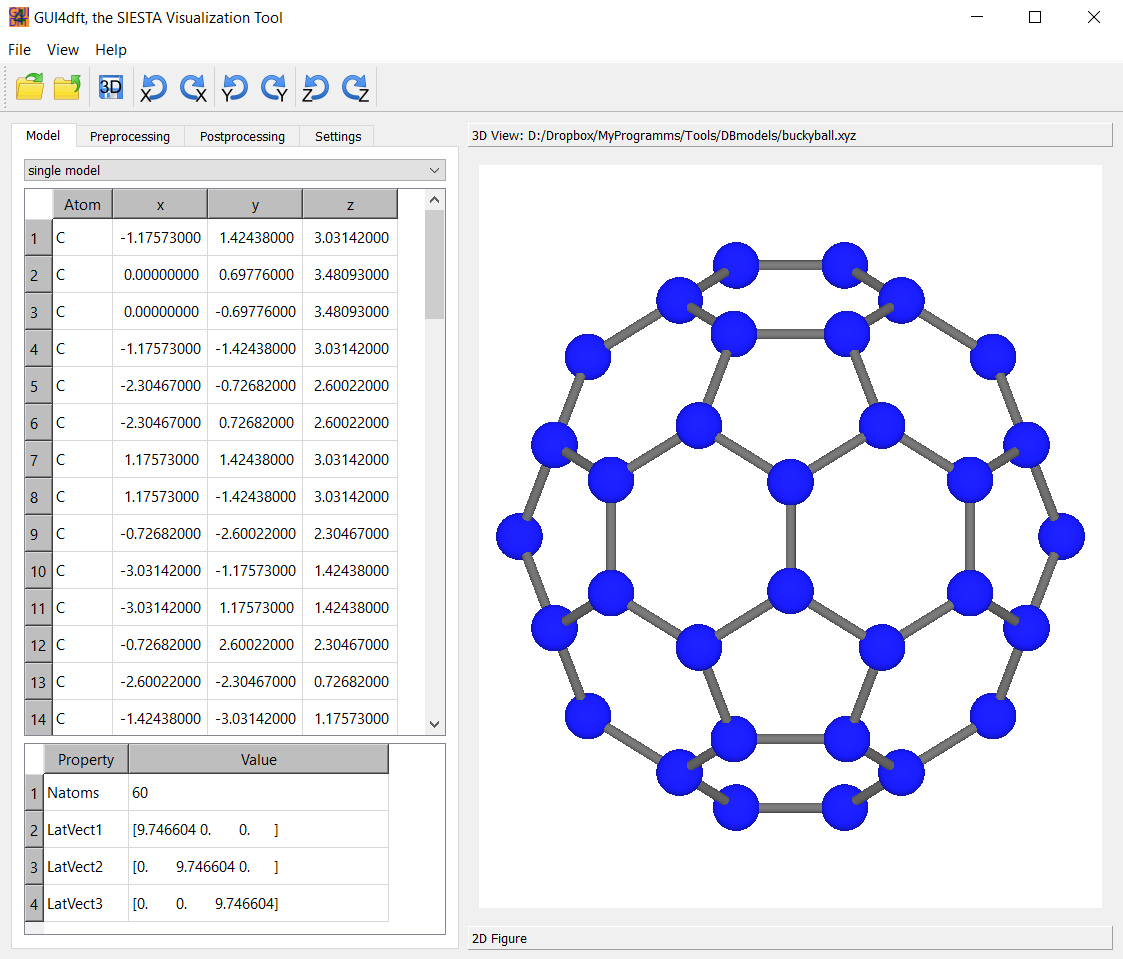
\includegraphics[width=5.0in]{mainwindow}
	\caption{Main window}
	\label{fig:mainwindow}
\end{figure}

\section{Installation}
GUI4DFT program is written in Python 3. It has some dependencies. Most of them are installed by default when using the anaconda toolkit \\(https://www.anaconda.com).

If you are using a python distribution kit from the https://www.python.org/ website, you need to execute \\ 
sudo pip3 install pyqt5 numpy scipy pyopengl matplotlib scikit-image \\
In Ubuntu do extra\\
sudo apt-get install qt5-default
	
\section{GUI}

The program combines a set of tools for preparing an input file for a SIESTA package and for post-processing of calculation results. The main window of the program consists of several parts (see Fig.\ref{fig:mainwindow}). On the left side of the screen are tabs Model, Preprocessing, Postprocessing and Settings. On the right side of the screen, 3D models and graphs are displayed.
	
\subsection{Model}

This tab displays general information about the atomic model: coordinates of atoms, vectors of a unit cell. If the file you are viewing contains information about several steps of atomic structure optimization, you can view each of them. The available atomic structures are shown in the drop-down list at the top of the section.

\subsection{Preprocessing}
\subsubsection{Create}

This tab allows you to create models of carbon nanotubes, graphene, as well as combine electrode models with the model under study (Fig. \ref{fig:precreate}).

\begin{figure}[h!]
	\centering
	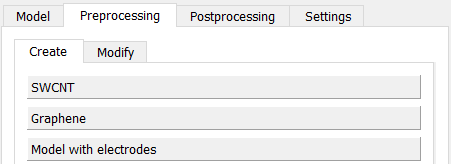
\includegraphics[width=10.0cm]{precreate}
	\caption{Tab Create}
	\label{fig:precreate}
\end{figure}

\textbf{SWNT}

The program allows you to create models of nanotubes with open ends (any chirality indices), with one or two closed ends (only for nanotubes (6,6) and (10,0)). When creating models of nanotubes with closed ends, it is required to indicate the rotation angles for the caps and the distance from the caps to the nanotube atoms. The user can specify the length of the model in angstroms or in the unit cell length.


\textbf{Graphene}

The size of the created graphene model is set by two integers defining one of the graphene boundaries and the length of the model in the direction perpendicular to this boundary.

\textbf{Model with electrodes}

To study the transport properties, it is necessary to prepare a model consisting of two electrodes and the studied atomic system. The graphical interface allows you to specify *.fdf files containing a description of the atomic structure of each of the three parts. The user can set the distance from the electrodes to the investigated fragment, as well as the angle of rotation of the investigated fragment.

\subsubsection{Modify}

This tab contains tools for modifying the viewed atomic structure and preparing the input file for the SIESTA package (Fig. \ref{fig:premodify}).

\begin{figure}[h!]
	\centering
	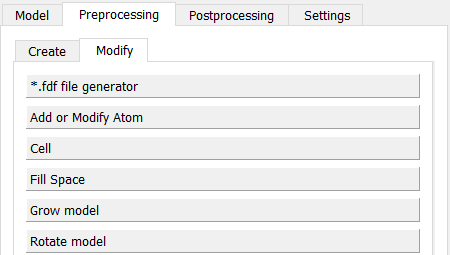
\includegraphics[width=10.0cm]{premodify}
	\caption{Tab Modify}
	\label{fig:premodify}
\end{figure}


\textbf{*.fdf file generator}

This tab allows you to prepare an input file for the SIESTA package. If the atomic system displayed in the program is obtained from a fdf file or the output stream of the SIESTA package, the generated text is ready for launch. Otherwise, only information related to the atomic structure is available.

The formats for the representation of translation vectors and atomic coordinates are configured on the tab described in the section \ref{settingsmode}.

The text is created by clicking the Generate button. This text can be edited directly in the program or saved to a file by clicking on the Save button.

\textbf{Add or Modify Atom}

This tab allows you to change or delete the selected atom. You can also add an atom to the structure (you cannot create a new model in this way, the atom is added to the existing model).

\textbf{Cell}

This tab allows you to redefine the translation vectors of the model. Coordinates are not recalculated, since the positions of atoms are stored in Cartesian coordinates inside the program. The changes made will only have an effect when exporting the structure in fractional coordinates.

\textbf{Fill Space}

This tab is designed to create cylinders of a given radius and length filled with atoms. The user can set the radius of the sphere surrounding the atom, which is not available for the centers of other atoms. The algorithm creates a series of such models, the degree of difference of which is specified by the delta parameter.

\textbf{Grow model}

This tab allows you to increase the size of the model along the x, y or z axes by translating.


\textbf{Rotate model}

This tab allows you to rotate the model by a specified angle (in degrees) around the axes of the Cartesian coordinate system. This rotation will affect the positions of the atoms when exported from the program.


\subsection{Postprocessing}

This tab contains several sections (Fig. \ref{fig:post}).

\begin{figure}[h!]
	\centering
	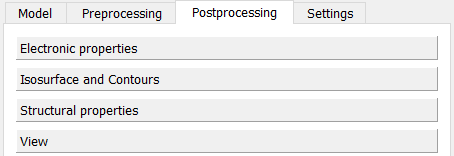
\includegraphics[width=10.0cm]{post}
	\caption{Tab Postprocessing}
	\label{fig:post}
\end{figure}

When opening the files of the SIESTA output stream, the presence of additional output files in the same directory is checked and the possibility of carrying out the corresponding analysis is activated. 

\subsubsection{Electronic properties}

\textbf{Band structure}

When you click on the "parse BANDS" button, a text file indicated in the text field above the button (it is filled in automatically) is analyzed. As a result the program displays the available ranges of k and energies. This range can be narrowed down for more informative drawings.

In addition, you can specify whether you want to show the Fermi level on the graph and shift the graph so that the Fermi level corresponds to zero energy.

\textbf{DOS}

On this tab, you can configure the density of states: show and position of the Fermi level, spin. In addition, you can add several datasets to one graph (by opening the file of the output stream of SIESTA).

\textbf{PDOS}

Partial density of states tools are located on two tabs. The first of them allows you to set filters by sort of atoms, number of atoms, quantum numbers, customize the the Fermi level and spin. The plotted graph is added to the list (you can specify the displayed label) located on the second tab. On the second tab, you can select the data sets to show on the figure.



\subsubsection{Isosurface and Contours}

The set of tools collected in this section allows you to visualize data in the XSF and cube formats.

\textbf{Data 1}

On this tab, the required file is selected (the list contains *.XSF and *.cube files of the current directory). When you click on the "Parse" button, the available datasets are displayed in the tree structure below. You need to select one of them and click the "Load Data" button. The data range is then displayed in the "Values" field.


\textbf{Data 2}

This tab is intended for calculating the sum or difference of two data sets with the possibility of further visualization or export to a file. If the operation has been performed, further actions are performed on the result of this operation.

Important: an operation with data is allowed only if the dimensions of the grids coincide.


\textbf{Isosurface}

On this tab, you can customize the displayed isosurfaces. By default, the isosurface color corresponds to the color scheme described in section \ref{colorsisos}. The color of the isosurface can be redefined by double-clicking on the corresponding position in the isosurfaces list. Transparency can be set independently for each isosurface.

\textbf{Contours}

On this tab, you can configure the display of flat sections of the displayed values (RHO, DRHO, etc.). The planes are perpendicular to the coordinate axes.


\subsubsection{Structural properties}

\textbf{Bonds}

This tab allows you to display bond lengths in the model and plot the corresponding histogram.

\textbf{Cell parameter}

This tab allows you to determine the equilibrium volume (or the translation along one of the axes) from a series of calculations with different parameters of the unit cell. The approximation can be carried out using the equations of Murnaghan, Birch-Murnaghan, or quadratic dependence.

\textbf{Selection history}

When sequentially selecting two atoms, the distance between them is displayed on the tab.

When three atoms are selected successively, the angle formed by them is displayed on the tab.

\textbf{Voronoi}

This tab allows you to plot a Voronoi polyhedron for a selected atom.

\subsubsection{View}

This tab allows you to color the atoms in accordance with their property (Milliken, Voronoi or Hirschfield charges). This option is only available for equilibrium configuration and if the corresponding property has been calculated.

Some of the atoms by their coordinates can be assigned to a fragment that will be displayed as semitransparent.


\subsection{Settings}

This tab contains several sections (Fig. \ref{fig:settings}).

\begin{figure}[h!]
	\centering
	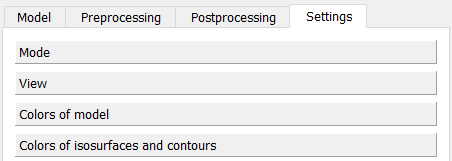
\includegraphics[width=10.0cm]{settings}
	\caption{Tab Settings}
	\label{fig:settings}
\end{figure}

All changes made on this tab are saved automatically and restored on subsequent program launches.

\subsubsection{Mode \label{settingsmode} }

The tab allows you to customize the mode of the program (the most important features of the work).

\textbf{Get only optimal structures}. If this option is selected, the program displays information only about the equilibrium model from the SIESTA output file.


\textbf{Parse atomic properties}. If this option is selected and the output file contains the charges of atoms (Milliken, Voronoi and Hirshfeld), these charges will be displayed in the Postprocessing $\to$ Structural properties $\to$ Selection history tab and can be used to color atoms in the system (Postprocessing $\to$ View).


\textbf{Allow atom selection}. If this option is selected, atoms can be selected using the mouse.


\textbf{Preferred coordinates}. This option defines the way of specifying coordinates in the *.fdf file (Postprocessing $\to$ Modify $\to$ *.fdf file generator): "Zmatrix Cartesian" or "Fractional".


\textbf{Preferred lattice}. This option defines the way of specifying the elementary cell in the *.fdf file.


\subsubsection{View}

On this tab, you can specify which elements of the model should be displayed (atoms, box, bonds, axes of the coordinate system) as well as set the thickness of interatomic bonds and isosurface lines (see Postprocessing $\to$ Isosurface and Contours $\to$ Contours).

\subsubsection{Colors of model}

To set the color of the atom, click on the corresponding row and select the color from the drop-down menu.

\subsubsection{Colors of isosurfaces and contours \label{colorsisos} }

This tab allows you to define the details of the display of isosurfaces and contours created on the tabs Postprocessing $\to$ Isosurface and Contours $\to$ Isosurface and Postprocessing $\to$ Isosurface and Contours $\to$ Contours.

The option "Color scheme" allows you to select a color scheme for the displayed physical values.


The option "Scale" allows you to choose between linear and logarithmic scales for defining isosurfaces.


The option "Contour color" sets the color of the isosurface lines in mode "Planes+Contours" (see Postprocessing $\to$ Isosurface and Contours $\to$ Contours).


The option "Use fixed colors range" allows you to use the same colors for several images, regardless of the range of values in these images. This can be useful for presenting the results in an article.


\section{Conclusion}
	All comments on the work of the program, please send to the email address sozykinsa@susu.ru
	
\bibliography{bibdatabase}
	
\end{document}